% Generated by src/run_section4.py -- every number comes from results/ at this commit.
% Needs \usepackage{graphicx}. Upload figures/s4_threshold.pdf to figures/.

\begin{table}[!htb]
\centering
\caption{Verification performance with counts (1,120 genuine and 49,920 impostor pairs; IoM uses shared key 0). Rates are FM/49,920 and FNM/1,120. Each EER row gives the EER and the two rates at the threshold where FMR and FNMR are closest; the EER is their mean. Bozorth3 scores are integers, so its FMR cannot hit 1\% or 0.1\% exactly.}
\label{tab:s4-counts}
\footnotesize
\setlength{\tabcolsep}{3pt}
\begin{tabular}{llrrr}
\hline
System & Point & Thr. & FMR \% (FM) & FNMR \% (FNM) \\
\hline
DeepPrint & EER = 6.25\% & 0.705 & 6.25 (3,120) & 6.25 (70) \\
 & \textbf{FMR 1\%} & 0.841 & 1.00 (499) & 18.93 (212) \\
 & FMR 0.1\% & 0.930 & 0.10 (49) & 58.57 (656) \\
\hline
NBIS & EER = 9.03\% & 11 & 9.76 (4,871) & 8.30 (93) \\
 & \textbf{FMR 1\%} & 18 & 0.69 (344) & 15.62 (175) \\
 & FMR 0.1\% & 24 & 0.07 (36) & 22.23 (249) \\
\hline
GRP-IoM & EER = 6.56\% & 111 & 6.59 (3,291) & 6.52 (73) \\
 & \textbf{FMR 1\%} & 155 & 1.00 (498) & 20.80 (233) \\
 & FMR 0.1\% & 202 & 0.09 (47) & 62.41 (699) \\
\hline
URP-IoM & EER = 6.10\% & 116 & 6.04 (3,017) & 6.16 (69) \\
 & \textbf{FMR 1\%} & 198 & 0.98 (490) & 20.00 (224) \\
 & FMR 0.1\% & 311 & 0.09 (46) & 61.70 (691) \\
\hline
\end{tabular}
\end{table}

\begin{figure}[!ht]
  \centering
  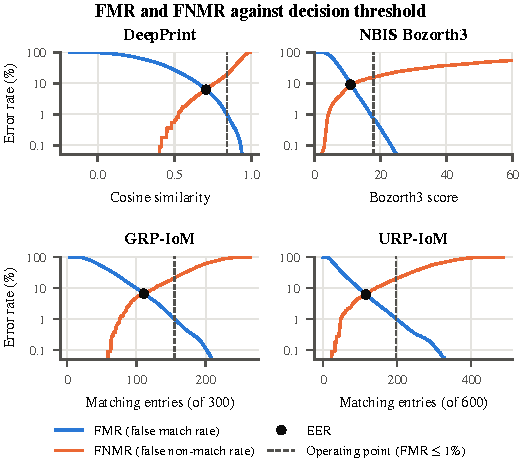
\includegraphics[width=\columnwidth]{figures/s4_threshold.pdf}
  \caption{\textbf{Threshold analysis.} FMR falls and FNMR rises as the threshold increases; the curves cross at the EER (dot). The dashed line marks the chosen operating point, FMR $\le$ 1\%, for every system (0.69\% for Bozorth3, whose scores are integers). The Bozorth3 axis is cut at 60; its FNMR reaches 100\% at the maximum score of 363.}
  \label{fig:s4-threshold}
\end{figure}

\begin{table}[!htb]
\centering
\caption{Where the baselines fail at FMR $\le$ 1\%: false non-matches per DB (of 280 genuine pairs) and false matches between different fingers of the same DB (of 2,880 pairs; cross-DB: of 38,400). Values: count (\%).}
\label{tab:s4-errors}
\footnotesize
\setlength{\tabcolsep}{2.5pt}
\begin{tabular}{lcccc}
\hline
 & \multicolumn{2}{c}{False non-matches} & \multicolumn{2}{c}{False matches} \\
DB & DeepPrint & NBIS & DeepPrint & NBIS \\
\hline
DB1 & 58 (20.7) & 57 (20.4) & 211 (7.3) & 38 (1.3) \\
DB2 & 109 (38.9) & 75 (26.8) & 2 (0.1) & 41 (1.4) \\
DB3 & 3 (1.1) & 20 (7.1) & 157 (5.5) & 45 (1.6) \\
DB4 & 42 (15.0) & 23 (8.2) & 36 (1.2) & 49 (1.7) \\
Cross-DB & -- & -- & 93 (0.2) & 171 (0.4) \\
\hline
\end{tabular}
\end{table}
